\chapter{Deployment Practices and System Observability}
\label{ch:production-pipeline}

Djøf Trade Union's deployment pipeline functions reliably but reveals opportunities for improvement. They manually approve each deployment stage, tests sometimes fail unpredictably, and monitoring gaps delay problem detection \textbf{(Transcript: 00:37:52)}.

\section{Current Pipeline and Monitoring Assessment}
\label{sec:current-pipeline}

Their current pipeline moves code through dev, test, and production environments \textbf{(Transcript: 00:31:37--00:32:07)}. Automated builds run unit tests, integration tests, and static analysis. However, deployment requires manual approval at each stage \textbf{(Transcript: 00:34:07--00:34:37)}.

Tests occasionally fail without reason and require reruns \textbf{(Transcript: 00:37:52)}. This instability wastes developer time and erodes confidence in test results. When tests fail randomly, they can't distinguish real problems from false alarms.

% Figure: Pipeline Current vs Recommended State
% Comparison of deployment pipeline practices

\begin{figure}[htbp]
    \centering
    \resizebox{0.9\textwidth}{!}{%
    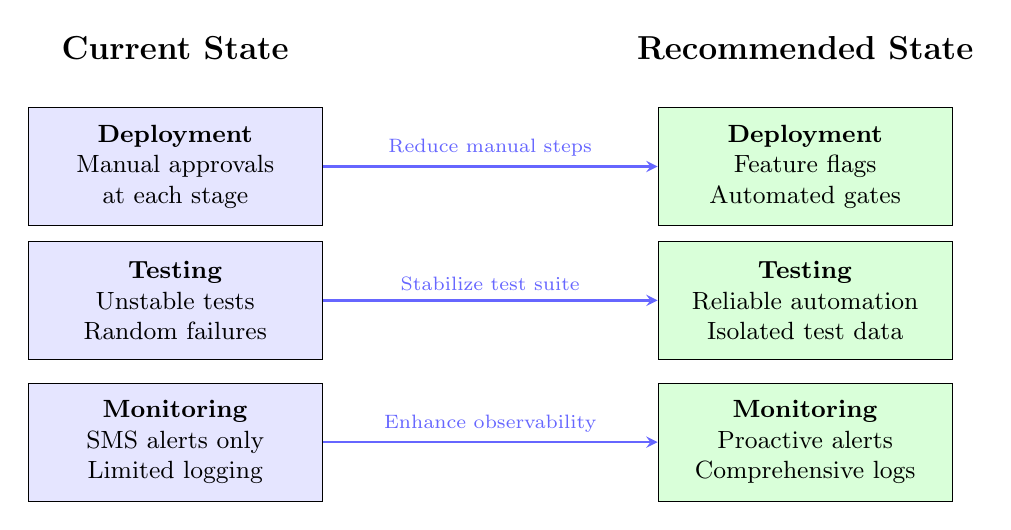
\begin{tikzpicture}[
        box/.style={rectangle, draw, fill=blue!10, text width=3.5cm, align=center, minimum height=1.5cm, font=\small},
        goodbox/.style={rectangle, draw, fill=green!15, text width=3.5cm, align=center, minimum height=1.5cm, font=\small},
        title/.style={font=\bfseries\large},
        arrow/.style={->, >=stealth, thick}
    ]

    % Current State (Left)
    \node[title] (current) at (0,5) {Current State};

    \node[box] (c1) at (0,3.5) {\textbf{Deployment}\\Manual approvals\\at each stage};
    \node[box] (c2) at (0,1.8) {\textbf{Testing}\\Unstable tests\\Random failures};
    \node[box] (c3) at (0,0) {\textbf{Monitoring}\\SMS alerts only\\Limited logging};

    % Recommended State (Right)
    \node[title] (recommended) at (8,5) {Recommended State};

    \node[goodbox] (r1) at (8,3.5) {\textbf{Deployment}\\Feature flags\\Automated gates};
    \node[goodbox] (r2) at (8,1.8) {\textbf{Testing}\\Reliable automation\\Isolated test data};
    \node[goodbox] (r3) at (8,0) {\textbf{Monitoring}\\Proactive alerts\\Comprehensive logs};

    % Connecting arrows with improvement labels
    \draw[arrow, blue!60] (c1) -- node[above, font=\scriptsize] {Reduce manual steps} (r1);
    \draw[arrow, blue!60] (c2) -- node[above, font=\scriptsize] {Stabilize test suite} (r2);
    \draw[arrow, blue!60] (c3) -- node[above, font=\scriptsize] {Enhance observability} (r3);

    \end{tikzpicture}%
    }
    \caption{Comparison of current and recommended pipeline practices. Current state relies on manual approvals and reactive monitoring. Recommended improvements focus on automation, test stability, and comprehensive observability to enable faster feedback and reduce operational overhead.}
    \label{fig:jawad-pipeline-comparison}
\end{figure}


Monitoring relies on SMS alerts for critical failures \textbf{(Transcript: 00:36:37)}. If problems occur overnight, the team discovers them the next morning. Limited logging makes root cause analysis difficult \textbf{(Transcript: 00:37:52--00:38:22)}.

The most impactful improvement would be comprehensive logging and monitoring \textbf{(Transcript: 00:38:37)}. Detailed logs capture system behavior. Proactive alerts detect anomalies before they escalate. This reduces response time and prevents user impact.

\section{Test Stability Improvements}
\label{sec:test-stability}

Stabilizing tests eliminates false failures. Isolating test data, managing test dependencies, and identifying flaky tests creates reliable automation. When teams trust their tests, they deploy confidently.

Gradually reducing manual approvals accelerates deployment. Feature flags enable safe production releases without manual gates. Teams can toggle features independently from deployment.

\section{Building Deployment Capabilities}
\label{sec:deployment-capabilities}

Enhanced observability transforms operations. Distributed tracing reveals request flows across services. Centralized logging aggregates data for analysis. Custom dashboards surface critical metrics in real time.

Improving deployment frequency builds organizational capability. More frequent deployments reduce batch size, making problems easier to diagnose and fixes faster to deploy.

Investing in test infrastructure pays dividends. Container-based test environments ensure consistency. Parallel test execution reduces feedback time. Regular test suite maintenance removes obsolete tests.
